\documentclass[conference]{IEEEtran}
\usepackage[T1]{fontenc}
\usepackage{lmodern}
\usepackage{graphicx}
\graphicspath{{img/}{tp1/docs/img/}}
\usepackage{booktabs}
\usepackage{amsmath}
\usepackage{amssymb}
\usepackage{float}
\usepackage{hyperref}
\usepackage{tikz}
\usetikzlibrary{arrows.meta}
\setlength{\emergencystretch}{1.5em}

\title{OS202 -- TD2: Mandelbrot, matrix--matrix product, and parallelism}
\author{Santiago Florido Gomez}

\begin{document}
\maketitle

\begin{abstract}
This document summarizes the TD1 work on weighted graphs: computing shortest paths by
minimum distances (Dijkstra, Bellman--Ford, Roy--Warshall) and building minimum spanning
trees with Kruskal. The algorithms are implemented and applied to the provided graphs.
\end{abstract}

\section{Introduction}
This report focuses on the TD1 exercises ``Spanning trees and shortest paths''.
We model the problems as weighted graphs and implement algorithms to identify shortest
paths by computing minimum distances and reconstructing paths between nodes. The study
covers Dijkstra (single-source with non-negative weights), Bellman--Ford (graphs that may
include negative weights), Roy--Warshall (all-pairs shortest paths), and Kruskal (minimum
spanning trees for cost-efficient connectivity). The implementations are validated on the
provided graphs (bank branch network and flight connections), and we briefly discuss the
assumptions and complexity of each algorithm.

\section{Trees}


\begin{figure}[H]
  \centering
  \includegraphics[width=0.55\linewidth]{img/exo1.png}
  \caption{Bank network with 7 branches and construction costs for each link (Exercise 1).}
  \label{fig:estructura-d3-banco-con-7-sucursales}
\end{figure}

Kruskal is used for finding the minimum spanning tree of the structure presented in Figure~ \ref{fig:estructura-d3-banco-con-7-sucursales}.
\begin{table}[H]
  \centering
  \small
  \resizebox{\linewidth}{!}{%
  \begin{tabular}{|c|c|c|c|c|c|c|c|c|c|c|c|c|}
\hline
\textbf{Edge}   & ab & bc & cd & bd & de & ed & ef & ca & bf & fg & ge & gd \\
\hline
\textbf{Weight} &  1 &  2 &  4 &  5 &  6 &  7 &  8 &  8 &  9 & 10 & 11 & 12 \\
\hline
\textbf{k}      &  1 &  2 &  3 &  X &  4 &  X &  5 &  X &  X &  6 &  X &  X \\
\hline
  \end{tabular}%
  }
\end{table}

\vspace{0.5em}

The main problem with the proposed structure is that, when finding the minimum spanning tree using Kruskal's algorithm, redundancy in the connections between different branches is eliminated, due to the absence of cycles that characterizes the tree resulting from Kruskal's application. For this reason, if a branch or an edge between branches fails, the bank's system would stop functioning (or become partially disconnected) from that point onward in the proposed spanning tree.

\begin{figure}[H]
  \centering
  \includegraphics[width=0.9\linewidth]{img/exo3.png}
  \caption{Graphs for finding minimal spanning trees with Kruskal.}
  \label{fig:graphs-for-finding-minimal-with}
\end{figure}

The following edge sets correspond to the results obtained by applying Kruskal's algorithm to build the
\emph{minimum spanning tree} (MST) of the graphs shown in Figure~\ref{fig:graphs-for-finding-minimal-with}.
In each case, Kruskal's method sorts all edges by non-decreasing weight and then iteratively adds the cheapest
edge that connects two different connected components, avoiding the creation of cycles. The resulting MSTs are:

\begin{itemize}
  \item \textbf{Image 1 (MST with Kruskal):}
  \[
  \begin{aligned}
  \{&(a,f,6.0),\ (b,e,5.0),\ (c,d,2.0),\ (c,g,5.0),\\
    &(e,f,1.0),\ (e,g,3.0),\ (g,h,5.0)\}
  \end{aligned}
  \]

  \item \textbf{Image 2 (MST with Kruskal):}
  \[
  \begin{aligned}
  \{&(A,C,3.0),\ (B,F,2.0),\ (C,D,2.0),\\
    &(D,F,3.0),\ (E,F,3.0)\}
  \end{aligned}
  \]
\end{itemize}

The following edge sets correspond to the results obtained by applying Kruskal's algorithm to compute the \emph{maximum spanning tree} (MAXT) of the graphs shown in Images 1 and 2. In this maximization variant, all edges are sorted by \emph{non-increasing} (decreasing) weight and the algorithm iteratively adds the heaviest edge that connects two different connected components, while still avoiding the creation of cycles. The resulting maximum spanning trees are:

\begin{itemize}
  \item \textbf{Image 1 (MAXT with Kruskal):}
  \[
  \begin{aligned}
  \{&(a,b,9.0),\ (a,f,6.0),\ (a,h,9.0),\ (b,d,8.0),\\
    &(b,e,5.0),\ (c,g,5.0),\ (d,g,8.0)\}
  \end{aligned}
  \]

  \item \textbf{Image 2 (MAXT with Kruskal):}
  \[
  \begin{aligned}
  \{&(A,B,4.0),\ (B,C,5.0),\ (C,F,5.0),\\
    &(D,E,4.0),\ (E,F,3.0)\}
  \end{aligned}
  \]
\end{itemize}

\section{Paths}

\begin{figure}[H]
  \centering
  \includegraphics[width=0.85\linewidth]{img/exo2.png}
  \caption{Travel time (in hours) between European cities.}
  \label{fig:paths-european-cities}
\end{figure}

Using Dijkstra for obtaining the shortest path from Paris to Rana in the graph of Figure~\ref{fig:paths-european-cities} we obtain the following.

\begin{table}[H]
  \centering
  \small
  \resizebox{0.7\columnwidth}{!}{%
  \begin{tabular}{|c|c|c|c|c|c|c|c|c|c|}
\hline
$i$ & pivot & H & A & L & B & O & E & S & R \\
\hline
-- & -- & $\infty$ & $\infty$ & $\varnothing$ & $\varnothing$ & $\varnothing$ & $\varnothing$ & $\varnothing$ & $\varnothing$ \\
\hline
1 & P & 7 & 3 & 4 &  &  &  &  &  \\
\hline
2 & A & 5 &  & 4 &  & 11 &  &  &  \\
\hline
3 & L &  &  &  &  &  & 6 &  &  \\
\hline
4 & H &  &  &  & 6 &  &  & 6 &  \\
\hline
5 & E &  &  &  &  &  &  &  & 12 \\
\hline
6 & D &  &  &  &  & 9 &  &  &  \\
\hline
7 & S &  &  &  &  & 8 &  &  & 11 \\
\hline
8 & O &  &  &  &  &  &  &  & 10 \\
\hline
  \end{tabular}%
  }
\end{table}

\bigskip

\begin{table}[H]
  \centering
  \small
\resizebox{0.7\columnwidth}{!}{%
  \begin{tabular}{|c|c|c|c|c|c|c|c|c|}
\hline
\textbf{Pred} & H & A & L & B & O & E & S & R \\
\hline
             & A & P & A & H & S & L & H & O \\
\hline
  \end{tabular}%
  }
\end{table}

\bigskip

\[
P \to A \to H \to S \to O \to R
\]

The following results show the predecessor relationships obtained by applying Dijkstra's
algorithm from the source node \textit{r} to all nodes in Figure~\ref{fig:graphs-for-dijkstra}.

\begin{table}[H]
  \centering
  \small
  \caption{Left graph: predecessor tree from node \textit{r}.}
  \label{tab:dijkstra-left-predecessors}
  \begin{tabular}{@{}l@{}}
    \toprule
    \textbf{Edges in the shortest-path tree} \\
    \midrule
    r -- a (5.0) \\
    r -- b (4.0) \\
    b -- c (3.0) \\
    b -- g (9.0) \\
    c -- d (2.0) \\
    c -- f (6.0) \\
    d -- e (2.0) \\
    \bottomrule
  \end{tabular}
\end{table}

\begin{table}[H]
  \centering
  \small
  \caption{Right graph: predecessor tree from node \textit{r}.}
  \label{tab:dijkstra-right-predecessors}
  \begin{tabular}{@{}l@{}}
    \toprule
    \textbf{Edges in the shortest-path tree} \\
    \midrule
    r -- A (2.0) \\
    r -- G (3.0) \\
    A -- B (3.0) \\
    A -- F (1.0) \\
    B -- C (2.0) \\
    F -- D (4.0) \\
    G -- E (2.0) \\
    \bottomrule
  \end{tabular}
\end{table}

\begin{figure}[H]
  \centering
  \includegraphics[width=0.9\linewidth]{img/exo4.png}
  \caption{Directed graphs used for Dijkstra shortest-path computation.}
  \label{fig:graphs-for-dijkstra}
\end{figure}

\subsection{Weighted precedence graph using the Activity-on-Arc transformation}

We represent the scheduling instance as a directed weighted graph obtained from the precedence graph
by the \emph{vertex-splitting} (Activity-on-Arc) construction.
Let the original tasks be $D,a,b,c,d,e,f,g,h,i,F$, where $D$ and $F$ have zero duration.
For each task vertex $x\in\{a,\dots,i\}$ we create two vertices $x_1$ and $x_2$, and we replace the
task by the directed arc $(x_1,x_2)$ weighted by the duration of task $x$.
All precedence arcs from the original graph are preserved and assigned weight $0$:
if $x\to y$ in the original precedence graph, then we add $x_2\to y_1$ with weight $0$.
The start node $D$ is connected to the start vertices of tasks with no predecessors, and the end node $F$
is reached from the completion vertex of the last task.

\paragraph{Task arcs (durations).}
\[
\begin{aligned}
&a_1\to a_2(4),\quad b_1\to b_2(6),\quad c_1\to c_2(4),\quad d_1\to d_2(12),\\
&e_1\to e_2(24),\quad f_1\to f_2(10),\quad g_1\to g_2(7),\quad h_1\to h_2(10),\quad i_1\to i_2(3).
\end{aligned}
\]

\paragraph{Precedence arcs (weight $0$).}
\[
\begin{aligned}
&D\to a_1,\quad D\to c_1,\quad D\to d_1,\\
&c_2\to b_1,\quad c_2\to g_1,\\
&a_2\to e_1,\quad b_2\to e_1,\quad b_2\to f_1,\\
&d_2\to h_1,\quad f_2\to h_1,\quad g_2\to h_1,\\
&e_2\to i_1,\quad h_2\to i_1,\\
&i_2\to F.
\end{aligned}
\]
All these arcs have weight $0$.

\paragraph{Why the graph is acyclic.}
Every precedence arc encodes a strict \emph{finish-before-start} constraint.
A directed cycle would force some task to be completed before it can start, which is impossible.
Therefore, the resulting directed graph is acyclic.

\begin{figure}[h]
\centering
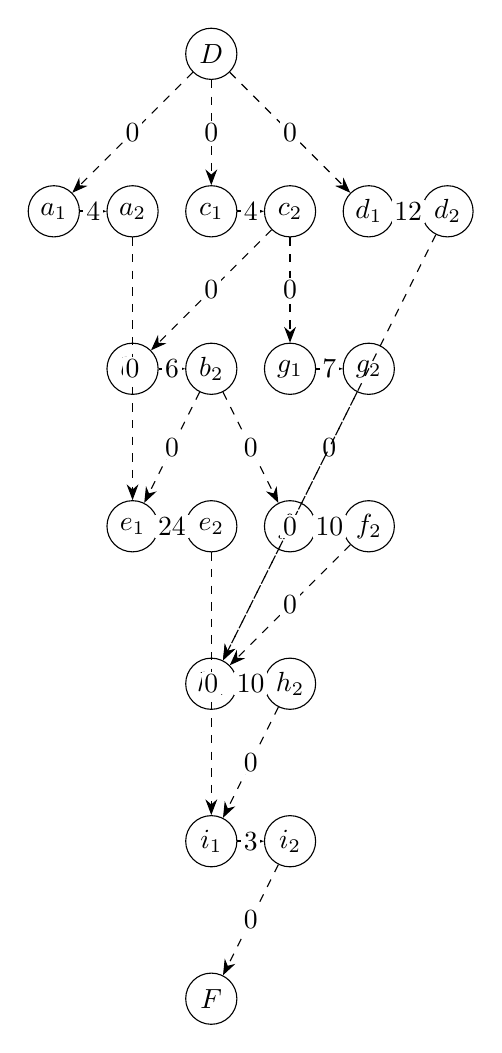
\begin{tikzpicture}[
  >=Stealth,
  v/.style={draw, circle, minimum size=6.5mm, inner sep=0pt},
  task/.style={-{Stealth[length=2mm]}, thick},
  prec/.style={-{Stealth[length=2mm]}, dashed},
  lab/.style={midway, fill=white, inner sep=1pt}
]

% --- Nodes (layered layout, vertical flow) ---
\node[v] (D)  at (0,0)  {$D$};

% Level 1: a,c,d (split)
\node[v] (a1) at (-2, -2) {$a_1$};
\node[v] (a2) at (-1, -2) {$a_2$};
\node[v] (c1) at (0,  -2) {$c_1$};
\node[v] (c2) at (1,  -2) {$c_2$};
\node[v] (d1) at (2,  -2) {$d_1$};
\node[v] (d2) at (3,  -2) {$d_2$};

% Level 2: b,g (split)
\node[v] (b1) at (-1, -4) {$b_1$};
\node[v] (b2) at (0,  -4) {$b_2$};
\node[v] (g1) at (1,  -4) {$g_1$};
\node[v] (g2) at (2,  -4) {$g_2$};

% Level 3: e,f (split)
\node[v] (e1) at (-1, -6) {$e_1$};
\node[v] (e2) at (0,  -6) {$e_2$};
\node[v] (f1) at (1,  -6) {$f_1$};
\node[v] (f2) at (2,  -6) {$f_2$};

% Level 4: h (split)
\node[v] (h1) at (0, -8) {$h_1$};
\node[v] (h2) at (1, -8) {$h_2$};

% Level 5: i (split) and end
\node[v] (i1) at (0, -10) {$i_1$};
\node[v] (i2) at (1, -10) {$i_2$};
\node[v] (F)  at (0, -12) {$F$};

% --- Task arcs (durations) ---
\draw[task] (a1) -- node[lab] {$4$} (a2);
\draw[task] (c1) -- node[lab] {$4$} (c2);
\draw[task] (d1) -- node[lab] {$12$} (d2);

\draw[task] (b1) -- node[lab] {$6$} (b2);
\draw[task] (g1) -- node[lab] {$7$} (g2);

\draw[task] (e1) -- node[lab] {$24$} (e2);
\draw[task] (f1) -- node[lab] {$10$} (f2);

\draw[task] (h1) -- node[lab] {$10$} (h2);
\draw[task] (i1) -- node[lab] {$3$} (i2);

% --- Precedence arcs (weight 0) ---
\draw[prec] (D) -- node[lab] {$0$} (a1);
\draw[prec] (D) -- node[lab] {$0$} (c1);
\draw[prec] (D) -- node[lab] {$0$} (d1);

\draw[prec] (c2) -- node[lab] {$0$} (b1);
\draw[prec] (c2) -- node[lab] {$0$} (g1);

\draw[prec] (a2) -- node[lab] {$0$} (e1);
\draw[prec] (b2) -- node[lab] {$0$} (e1);
\draw[prec] (b2) -- node[lab] {$0$} (f1);

\draw[prec] (d2) -- node[lab] {$0$} (h1);
\draw[prec] (f2) -- node[lab] {$0$} (h1);
\draw[prec] (g2) -- node[lab] {$0$} (h1);

\draw[prec] (e2) -- node[lab] {$0$} (i1);
\draw[prec] (h2) -- node[lab] {$0$} (i1);

\draw[prec] (i2) -- node[lab] {$0$} (F);

\end{tikzpicture}
\caption{Activity-on-Arc weighted graph: solid arcs represent tasks (duration as weight),
dashed arcs represent precedence constraints (weight $0$).}
\end{figure}

Since the constructed graph does not represent an optional route in which the change is located, but instead necessarily implies going through all stages, the minimum-cost calculation to go from \textbf{D} to \textbf{F} does not yield the expected result. However, because a task cannot start until its predecessors have finished, for tasks preceded by multiple nodes the earliest possible start time is necessarily equal to the completion time of the predecessor with the largest waiting time; that is, the \textbf{maximum} over its predecessors. Therefore, to determine the \textbf{minimum} duration of the entire project, it is convenient to identify the \textbf{maximum-duration path} between \textbf{D} and \textbf{F}, since this maximum is equivalent to that minimum required time.

\paragraph{Warshall computation (max-plus version).}
To obtain this longest path, we apply the Warshall/Floyd--Warshall algorithm by replacing
the $\min$ operator with $\max$ (and initializing missing arcs to $-\infty$):
\[
\text{dist}[i][j] \leftarrow \max\big(\text{dist}[i][j],\ \text{dist}[i][k]+\text{dist}[k][j]\big).
\]
The resulting \texttt{Distances} matrix directly gives the minimum project duration:
\[
\text{dist}(D,F)=37.
\]
Thus, the minimum project duration is \textbf{37} (in the weight units of the graph).

\paragraph{Critical path and critical tasks.}
The \texttt{Predecessors} matrix lets us reconstruct the path achieving this value:
\[
\begin{aligned}
D \;\to\; c_1 \;\to\; c_2 \;\to\; b_1 \;\to\; b_2 \;\to\; e_1 \;\to\; e_2\\
\to\; i_1 \;\to\; i_2 \;\to\; F.
\end{aligned}
\]
Along this path, the \emph{task} arcs (those of the form $x_1\to x_2$) have the following durations:
\[
\begin{aligned}
&c_1\to c_2(4),\qquad b_1\to b_2(6),\\
&e_1\to e_2(24),\qquad i_1\to i_2(3),
\end{aligned}
\]
so
\[
4+6+24+3=37.
\]
The \textbf{critical tasks} are therefore $\{c,b,e,i\}$, that is, the task arcs
$c_1\to c_2$, $b_1\to b_2$, $e_1\to e_2$, and $i_1\to i_2$ (any increase in their duration delays $F$).

\begin{figure}[h]
\centering
\resizebox{\columnwidth}{!}{%
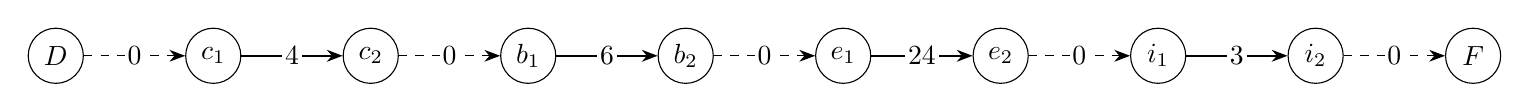
\begin{tikzpicture}[
  >=Stealth,
  v/.style={draw, circle, minimum size=7mm, inner sep=0pt},
  task/.style={-{Stealth[length=2mm]}, thick},   % critical task arcs (durations)
  prec/.style={-{Stealth[length=2mm]}, dashed},  % precedence arcs (weight 0)
  lab/.style={midway, fill=white, inner sep=1pt}
]
% Nodes (critical chain only)
\node[v] (D)  at (0,0)  {$D$};
\node[v] (c1) at (2,0)  {$c_1$};
\node[v] (c2) at (4,0)  {$c_2$};
\node[v] (b1) at (6,0)  {$b_1$};
\node[v] (b2) at (8,0)  {$b_2$};
\node[v] (e1) at (10,0) {$e_1$};
\node[v] (e2) at (12,0) {$e_2$};
\node[v] (i1) at (14,0) {$i_1$};
\node[v] (i2) at (16,0) {$i_2$};
\node[v] (F)  at (18,0) {$F$};

% Precedence arcs (weight 0)
\draw[prec] (D)  -- node[lab] {$0$} (c1);
\draw[prec] (c2) -- node[lab] {$0$} (b1);
\draw[prec] (b2) -- node[lab] {$0$} (e1);
\draw[prec] (e2) -- node[lab] {$0$} (i1);
\draw[prec] (i2) -- node[lab] {$0$} (F);

% Task arcs (durations) = critical tasks
\draw[task] (c1) -- node[lab] {$4$}  (c2);
\draw[task] (b1) -- node[lab] {$6$}  (b2);
\draw[task] (e1) -- node[lab] {$24$} (e2);
\draw[task] (i1) -- node[lab] {$3$}  (i2);

\end{tikzpicture}
}
\caption{Critical path (task arcs in bold) and precedence arcs (dashed, weight $0$).
Total duration: $37$.}
\end{figure}

\begin{figure}[h]
\centering
\resizebox{\columnwidth}{!}{%
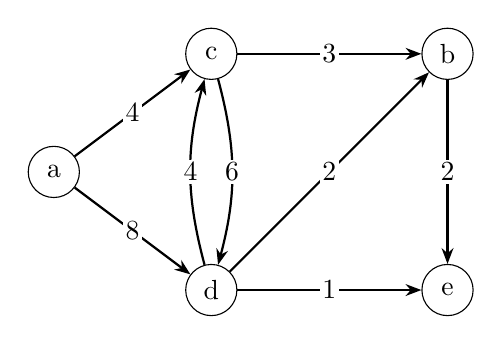
\begin{tikzpicture}[
  >=Stealth,
  v/.style={draw, circle, minimum size=6.5mm, inner sep=0pt},
  e/.style={-{Stealth[length=2mm]}, thick},
  lab/.style={midway, fill=white, inner sep=1pt}
]
\node[v] (a) at (0,0) {a};
\node[v] (c) at (2,1.5) {c};
\node[v] (d) at (2,-1.5) {d};
\node[v] (b) at (5,1.5) {b};
\node[v] (e) at (5,-1.5) {e};

\draw[e] (a) -- node[lab] {4} (c);
\draw[e] (a) -- node[lab] {8} (d);
\draw[e] (c) to[bend left=15] node[lab] {6} (d);
\draw[e] (d) to[bend left=15] node[lab] {4} (c);
\draw[e] (c) -- node[lab] {3} (b);
\draw[e] (d) -- node[lab] {2} (b);
\draw[e] (b) -- node[lab] {2} (e);
\draw[e] (d) -- node[lab] {1} (e);
\end{tikzpicture}
}
\caption{Directed graph (Exercise 6).}
\end{figure}

Since there is a cyclic section in the graph, the use of the Roy--Warshall (Floyd--Warshall) algorithm is proposed. The results are presented in the following table.

\bigskip

\noindent\textbf{Distances}
\[
\begin{array}{c|ccccc}
      & a & c & d & b & e\\ \hline
a     & 0 & 4 & 8 & 7 & 9\\
c     & \infty & 0 & 6 & 3 & 5\\
d     & \infty & 4 & 0 & 2 & 1\\
b     & \infty & \infty & \infty & 0 & 2\\
e     & \infty & \infty & \infty & \infty & 0
\end{array}
\]

\bigskip

\noindent\textbf{Predecessors}
\[
\begin{array}{c|ccccc}
      & a & c & d & b & e\\ \hline
a     & - & a & a & c & d\\
c     & - & - & c & c & b\\
d     & - & d & - & d & d\\
b     & - & - & - & - & b\\
e     & - & - & - & - & -
\end{array}
\]

\bigskip

\noindent\textbf{How to obtain the shortest paths from these tables}

\begin{itemize}
  \item The \textbf{Distances} matrix stores, at entry $(i,j)$, the minimum distance (cost) from $i$ to $j$.
  \item The \textbf{Predecessors} matrix stores, at entry $(i,j)$, the \emph{immediate predecessor} of $j$ on a shortest path from $i$ to $j$.
  \item To reconstruct the shortest path from $i$ to $j$:
  \begin{enumerate}
    \item If $\text{Distances}[i,j]=\infty$, then there is \textbf{no path} from $i$ to $j$.
    \item If $i=j$, the path is simply $(i)$.
    \item Otherwise, set $v \leftarrow j$ and build the path backwards by repeatedly applying
      \[
      v \leftarrow \text{Predecessors}[i,v]
      \]
      until reaching $i$.
    \item The shortest path is the resulting sequence, but read in \textbf{reverse order} (because it was built from $j$ back to $i$).
  \end{enumerate}
\end{itemize}

\bigskip

\noindent\textbf{Examples using your tables}

\begin{itemize}
  \item Shortest path from $a$ to $e$:  
  $\text{Predecessors}[a,e]=d$, then $\text{Predecessors}[a,d]=a$.  
  Hence the path is $a \rightarrow d \rightarrow e$ and its cost is $\text{Distances}[a,e]=9$.
  
  \item Shortest path from $a$ to $b$:  
  $\text{Predecessors}[a,b]=c$, and $\text{Predecessors}[a,c]=a$.  
  Path: $a \rightarrow c \rightarrow b$, cost $\text{Distances}[a,b]=7$.
  
  \item Shortest path from $c$ to $e$:  
  $\text{Predecessors}[c,e]=b$, and $\text{Predecessors}[c,b]=c$.  
  Path: $c \rightarrow b \rightarrow e$, cost $\text{Distances}[c,e]=5$.
\end{itemize}

\end{document}
